\documentclass[10pt,a4paper]{article}
\usepackage[latin1]{inputenc}
\usepackage[english]{babel}
\usepackage{amsmath}
\usepackage{amsfonts}
\usepackage{amssymb}
\usepackage{makeidx}
\usepackage{graphicx}
\usepackage{hyperref}
\usepackage[left=2cm,right=2cm,top=2cm,bottom=2cm]{geometry}


\author{Anders Dall'Osso Teigset}
\title{PUFFER MECHANISM SKRIV I STORE BOKSTAVER}

\begin{document}
\maketitle
%Summary
\newpage
\section{Summary}
\newpage
\tableofcontents
\newpage
\section{Introduction}
A load break switch should be able to interrupt currents less or equal the maximum load current in a distribution system. When interrupting a current the two contacts which a switch consists of start separating producing a gap between each other. Normally the current is not interrupted by this and an electrical arc ignites and burns in the contact gap \cite{bib:HVEbreak}. The arc consists of plasma, which is a mixture of negative and positive ions as well as electrons. Due to the energy dissipation produced by the arc the temperature in the plasma is very high. The electrical conductivity of the plasma channel is dependent of the temperature produced by the arc. When a high current is flowing it is almost a perfect conductor, but at low temperatures the conductivity is much poorer.

An AC-current have a natural zero crossing, as the current approaches this point the arc will start cooling and extinguish if properly cooled at this point of the power cycle. The working principle of a switchgear is to cool the arc sufficiently when the current approaches zero and then quench the arc when the current is zero. At this moment the current is interrupted and a voltage builds up across the open contacts. This voltage is called the recovery voltage. The steepness and amplitude of the recovery voltage \cite{bib:HVEbreak} and the design of the switchgear will decide if a new arc ignites between the contacts after the current zero. If an arc re-ignites ether by a thermal or a dielectric breakdown the interruption has failed. 

Upon till now SF$_6$ and vacuum based technology have been dominating the compact medium-voltage switchgear market. Air insulated switchgear does exists but they are space consuming and are not applicable for use in a compact substation design. A compact substation is one of the most common designs for substations in the medium-voltage level of the distribution system. Figure \ref{fig:compact substation} displays a compact substation which can be used in the medium-voltage distribution system. The switchgear is a module that can be detached from the compact substation and removed trough its front panel. As figure \ref{fig:compact substation} indicates there are a limited amount of space available for the switchgear. Therefore the main challenge for an air insulated switchgear design for this kind of application is set by the amount of space available in the compact substation.

\begin{figure} [h]
\centering
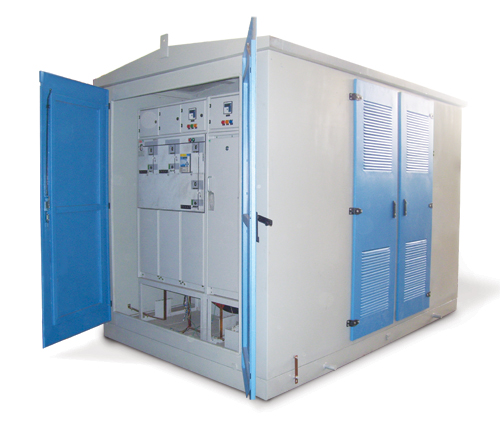
\includegraphics[scale=0.5]{Bilder/Introduction/general_substation.jpg}
\caption{Compact substation with open front panel \cite{bib:comSub}} \label{fig:compact substation}
\end{figure}

The main choice of interrupting media in switchgear has been SF$_6$ since its discovery in the 1970ies. The gas exhibits many properties which is well suited for an isolation gas. It is highly electron negative which gives it good dielectric strength and arc-interrupting capabilities. The breakdown voltage of SF$_6$ is almost three times higher than air at atmospheric pressure \cite{bib:SF6PI}. It has excellent heat transfer properties as an interrupting medium \cite{bib:SF6PI}. The gas also reforms itself when dissociated under the high temperature conditions in an electrical arc. SF$_6$ produces no polymerization, carbon or other conductive deposits during arcing. It is also chemically compatible with most insulation materials and conductive materials \cite{bib:SF6PI}. The gas is also well suited for use in low temperature environments since its boiling point is fairly low even at high pressures. The gas in its stable form is nontoxic, non-flammable and non-explosive. It is also thermally stable and do not decompose at normal operating temperatures for a closed switch \cite{bib:SF6PI}. SF$_6$ based switchgear tends to be cheap to produce relative to other designs, and the gas itself is also affordable at today prices.


SF$_6$ have some disadvantages, when exposed to electrical discharge or arcing it forms highly toxic and corrosive compounds \cite{bib:SF6PI}. It is also hard to remove non-polar contaminants like air and its breakdown voltage is sensitive to water vapour and conductive particles. However it biggest downside is probably that it is an effective infrared absorber. This makes it a strong greenhouse gas \cite{bib:SF6PI} and it is regarded to be almost $20000$ times as potent as CO$_2$.

0.4 \% of the greenhouse gas emissions in Norway is due to SF$_6$ and is mainly used in switchgear or other high voltage equipment \cite{bib:KlimaKur2020}. In Norway the use of SF$_6$ is regulated through a voluntary contract between the environmental department and the end user, mainly the power companies \cite{bib:KlimaKur2020}. If a compatible air based switchgear design is released on the market it can be assumed that the power companies will be interested in the new technology. It is also possible that the government will restrict the use of SF$_6$ gas if the private sector do not follow the guidelines of the environmental department.

A test switch have been developed which allows adjustment of many design parameter such as nozzle and contact geometry, contact movement and gas pressure. The contacts consist of one female contact, or tulip and one male contact, or pin. The tulip is immovable, while the pin can be opened by a spring trigged by an electromagnet. Previous results have illustrate that most of the successful interruptions have occurred when the pin is outside the nozzle \cite{bib:CIAMVLBS}. Cold air simulations done by Nina Sasaki Aanensen of the different geometries have stated that volumetric flow of air is much lower when the pin is inside the nozzle. The results from previous testing and cold air simulations might suggest that the pin is clogging the nozzle and preventing a good air flow. Therefore a new nozzle geometry has been designed with a doughnut area, the area between the nozzle and the pin, which is bigger than the area of the pin. This is assumed to give a volumetric flow of air that is almost the same when the pin is inside the nozzle as well as outside. The theory has been verified by cold air simulations. However the clogging effect generated by an arc has not been taken into account and it is expected that this will have an impact on the volumetric flow. Two nozzles have been constructed of the new nozzle geometry one with an doughnut area of $44 \ mm^2$ and the other one with an area of $66 \ mm^2$. It is expected that the speed of the air will be constant and the volumetric flow will increase with the doughnut area. This will give an opportunity to test which of these parameters that influence the current interruption capabilities the most.

Several different nozzle geometries are going to be tested and it is assumed that the chance for a successful current interruption inside the nozzle will be approximately the same as outside the nozzle. Since the size of the arc compared to the pin will vary between the different nozzle geometries and current amplitudes, a clogging effect is assumed to occur and might be revealed as an lower interruption success rate for certain geometries.

\newpage
\section{Theory}
\subsection{Switchgear design}
\subsubsection{General design} \label{sec:genDes}
Switchgear can be divided into four main categories:
\begin{itemize}
\item Disconnector Switch
\item Load Break Switch
\item Circuit Breaker
\item Earthing Switch
\end{itemize}
This report will focus on the load break switch (LBS) design. A LBS is a switchgear design to be able to interrupt currents with magnitude that is equal or less than the rated maximum continuous current in a transmission system. A LBS must fulfil the following demands to meet the requirements of the application area:

\begin{itemize}
\item When closed:
	\begin{itemize}
		\item It must act as an perfect conductor.
		\item Be capable to interrupt any currents that may arise, without generating too high over-voltages. 
	\end{itemize}
\item When open:
	\begin{itemize}
		\item It must be an perfect isolator.
		\item Be able to close without welding the contacts together, event under short-circuit conditions.
	\end{itemize}
\end{itemize}

In a LBS it is important to assure that the switch in closed position acts as a perfect conductor with low contact resistance. This will minimize electrical losses in the switch and therefore minimize economical losses. Copper or aluminium is ideal materials and are often used to ensure that this aspect of the contact is met. Sometimes the contact surface is plated with tin, gold, silver or platinum to ensure a low contact resistance between the contact plates. The main problem with electrical losses in the switch is heat generation which may speed up metal creeping processes and other ageing related processes in the switch. Contact plates made out of aluminium are especially vulnerable to creeping.
 
To withstand the harsh conditions that occurs when an arc burns between the contacts the contact material has to meet strict requirements. It has to tolerate high temperatures, arc erosion, welding and other stresses that may apply when closing or opening an energized contact. Aluminium and copper is not fit for these tasks since they will melt or erode from stresses of an arc. It is common to use composites of metals with good electrical conduction with heat resistant oxides. For high current and voltage switches it is usual to use a composite of silver or copper together with tungsten or tungsten carbide. These materials are very resistant against heat, erosion and welding, but they have a high resistance. Therefore it is common on breakers above $70 \ kV$ to have two sets of contacts, one arcing contact and one main contact. The main contact is the first contact to open and the last one to close. This is to ensure that an arc do not start to burn between the contact, which makes it possible to use aluminium or copper as contact materials. The arcing contact is the last contact to open, and the first one to close. This will ensure that the arc burns between the arcing contact and not between the main contact. This contact arrangement is also common in the compact LBS systems available today, and many other common switchgear designs.

To quench the arc several mechanisms and interrupting mediums can be applied. In today's compact LBS systems based on SF$_6$ the puffer mechanisms is commonly used. Details regarding arc quenching is explained in section \ref{sec:InterruptCurrent}. To obtain a successful interruption of an arc it is possible to cool the arc and interrupting gas down, as well as blow away charged particles and metal oxides between the contact points. This is the main goal with the puffer mechanism. As SF$_6$ entered the industry in the 1960s it was in the form of dual pressure breakers \cite{bib:HVEbreak}. The SF$_6$ based dual pressure breakers had one high pressure chamber, and one low pressure chamber. A valve from a high pressure chamber opens during opening operations, generating a high speed SF$_6$ blast, guided by a nozzle, to hit the arc burning between the contacts in the low pressure chamber. This design have two major disadvantages when using SF$_6$ instead of air. The switch requires heating to maintain the high pressure in the high pressure chamber so that the SF$_6$ gas do not condensates. It also uses a compressor to pump the gas from the low pressure chamber to the high pressure chamber. This adds to the complexity to the switchgear and may result in more maintenance. The double pressure design was replaced with the single pressure design. The single pressure design has only one pressure chamber with low pressure except during interruptions when the chamber it self becomes a high pressure reservoir \cite{bib:HVEbreak}.

The single pressure SF$_6$ switchgear is using the puffer or the self-blast mechanism to quench an arc, or in some cases a combination with both. Common for both puffer and self-blast mechanisms are that they do not use a compressor to generate the gas flow, but uses the energy stored in the switching mechanisms or generated from the blast itself to interrupt the arc \cite{bib:HVEbreak}. These mechanisms works the same way for both circuit breakers and load break switches, but will in a load break switch be smaller and less complex. This is because the current amplitudes are smaller and therefore a lower pressure is needed to obtain a successful interruption.

The puffer mechanism is based on a piston to generate a flow of gas in the switchgear to extinguish the arc. A typical design of this system is by using a fixed piston integrated as a part of the contact design \cite{bib:HVEbreak}. A gas reservoir trapped between the arcing contact and the piston is pushed out as the contact moves apart for each other. Figure \ref{fig:CircutBreakPuff1} displays a typical interruption sequence of a puffer design breaker.


\begin{figure} [h]
\centering
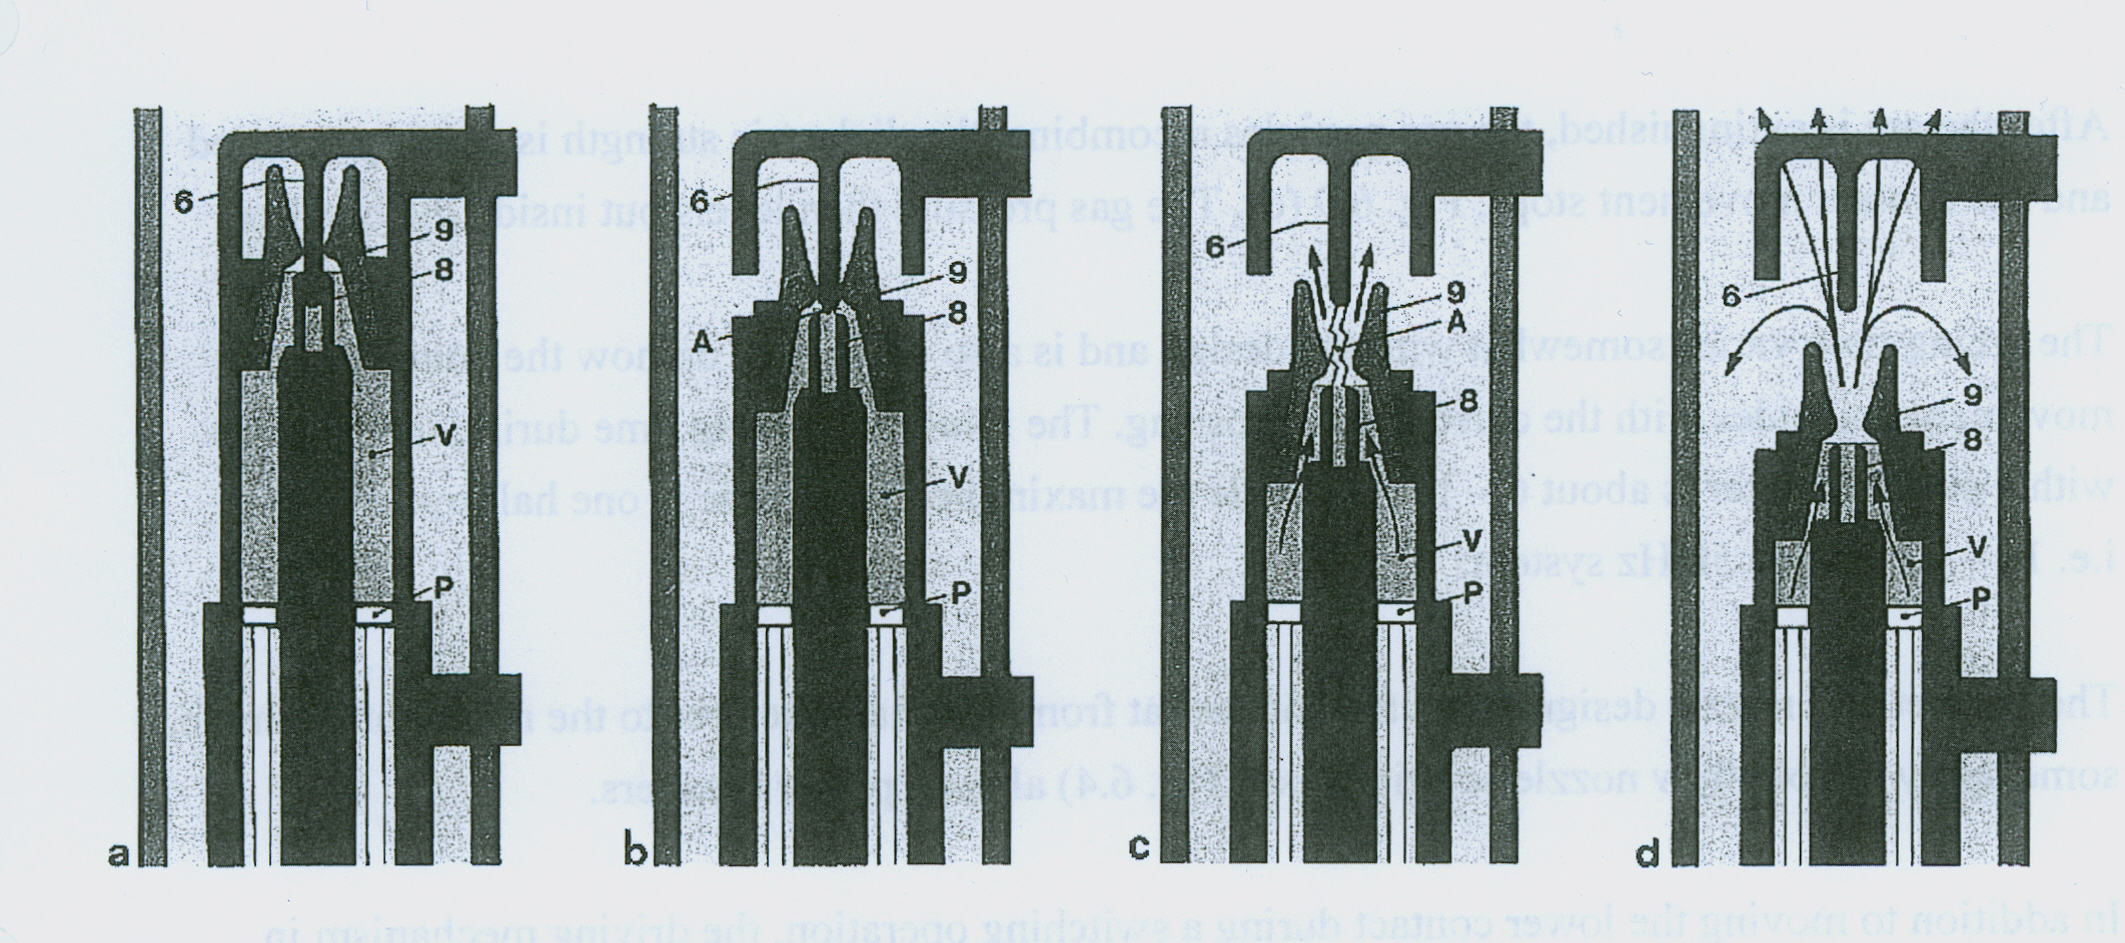
\includegraphics[scale=0.8]{Bilder/Theory/CircutBreakPuff1.png}
\caption{Interruption sequence in a puffer breaker \cite{bib:HVEbreak}} \label{fig:CircutBreakPuff1}
\end{figure}

When the breaker is closed as seen in figure \ref{fig:CircutBreakPuff1}a there is a gas volume \textit{(V)} trapped between the piston \textit{(P)} and the arcing contact \textit{(8) and (6)}. When the movable part of the arcing contact is pulled down the volume decreases because of the fixed piston. Then an increase in pressure due to compression of the gas occurs. Figure \ref{fig:CircutBreakPuff1}b illustrate that the main contact is open, and that the current now only flows through the arcing contact.

The next stage of the interruption sequence is pointed out in figure \ref{fig:CircutBreakPuff1}c. The arcing contacts have now separated and an arc \textit{(A)} has ignited between the contacts. The pressurised gas that previously was trapped between the piston and the arcing contact is now released. The gas flow is guided by a nozzle \textit{(9)} that is fixed to the movable arcing contact. The gas flow will cool down the arc and blow away charge carriers between the contact plates. If a sufficient gas flow is obtained the arc will not re-ignite after current zero and neither extinguish before current zero, so that current chopping is avoided.

The gas flow is partially dependent on the cross-section of the arc, which again is dependent on the current amplitude. A large current resulting in an large arc may block the hole in the nozzle preventing a gas flow. This is called current clogging and may occur for certain nozzle designs at high current interruptions. In such an event the pressure in the gas reservoir will increase further due to compression from mechanical moment of the arcing contact and thermal expansion in the gas because of heating from the arc. When the current amplitude approaches zero its cross-section will decrease and the clogging effect will end. This will result in a powerful gas blast onto the arc, as indicated in figure \ref{fig:CircutBreakPuff1}d. For smaller current amplitudes the arc cross-section is smaller and a blocking effect does not occur in the same extent. This generates a less intense gas flow, preventing current chopping.
 

\begin{figure} [h]
\centering
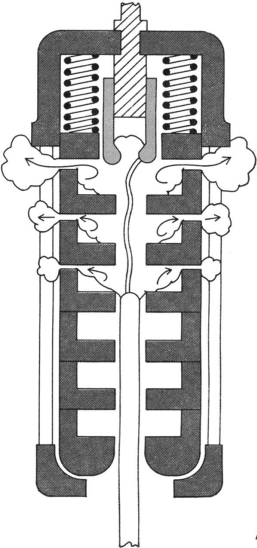
\includegraphics[scale=0.4]{Bilder/Theory/selfBlast.png}
\caption{Expulsion chamber in a breaker using the self-blast mechanism \cite{bib:CBAC}} \label{fig:selfBlast}
\end{figure}

The self-blast, or third generation breaker, was developed with the goal of reducing mechanical power of the operating system, making it cheaper and less complex. Figure \ref{fig:selfBlast} illustrates the working principle of a breaker using self-blast to interrupt an arc. The difference between self-blast and puffer mechanism is that the puffer mechanism increases the pressure by reducing the volume. Rather than the self-blast design which have a constant volume relying on a raise in temperature to increase the gas pressure \cite{bib:CBAC}. The self-blast design uses the heat generated from an arc burning between the arcing contacts to interrupt the current. The gas expands as it is heated by the burning arc, this increase in pressure leads to a gas flow on the arc, which cools it down leading to the quenching of it.

There are some disadvantages with the self-blast principle when compared to the puffer mechanism. The self-blast have a lower dielectric strength due to hot gas between the contacts after CZ. This gives a higher chance of re-ignition since hot gas has a higher conductivity than cold gas \cite{bib:HVEbreak}. It is also not well suited to break smaller currents. This is because the arc is less intense and therefore do not heat the gas sufficiently to create a strong enough blast. Because of this it is common to combine self-blast and puffer mechanism in a hybrid design, so that it can handle both small and large currents \cite{bib:HVEbreak}. A compact LBS design using air as interrupting medium will probably rely on a puffer or a hard gas design. This is because of the smaller currents an LBS is facing compared to a circuit breaker.


\subsubsection{Test switch}
A new medium voltage laboratory for load break switch development have been designed with the possibilities to vary important design parameters for a load break switch. When the industry develops switchgear technology they tend to alter several different parameters at the same time. For instance, if they wish to alter the speed of the airflow in a puffer LBS, they might increases the separation speed of the contacts, since these functions often are linked in a puffer design. This will also result in a higher pressure not only and not only a higher volumetric flow. This will make it hard to conclude which parameter that was the most critical for a successful interruption. Therefore a laboratory switch have been design where each of the different parameters can be adjusted without changing other critical parameter. This will make systematic researching possible and optimisation of certain designs criteria, like dimensions, will be a lot simpler.

\begin{figure} [h]
\centering
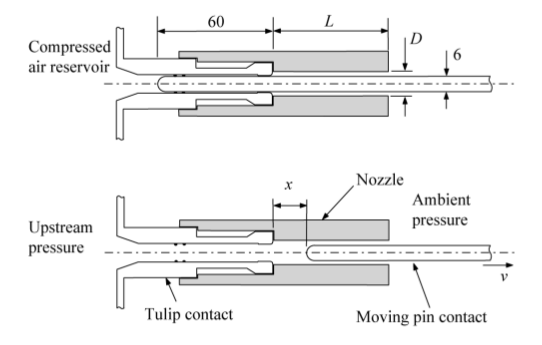
\includegraphics[scale=0.5]{Bilder/Theory/SchematicTestSwitch.png}
\caption{Test switch} \label{fig:testSwitch}
\end{figure}

Figure \ref{fig:testSwitch} shows the physical appearance of the switch and how the different parameter can be adjusted. BLA BLA TAKE A PICTURE OF THE SWITCH, WRITE SOME NUMBERS ON IT. TAKE ABOUT THEM AND WITCH PARAMETERS THAT CAN BE ADJUSTED.

\begin{figure} [h]
\centering
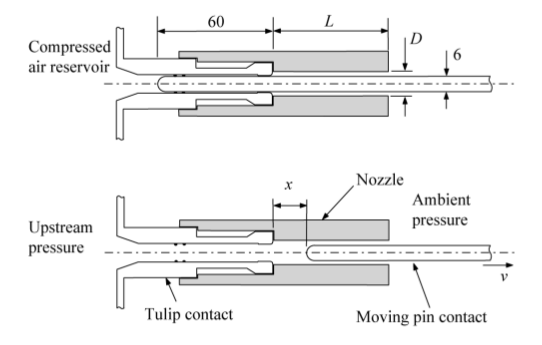
\includegraphics[scale=0.5]{Bilder/Theory/SchematicTestSwitch.png}
\caption{Tulip, nozzle and pin, L and D is the length and inner diameter of the nozzle, x is contact position. Dimensions are in millimetres.   \cite{bib:CIAMVLBS}} \label{fig:SchematicTestSwitch}
\end{figure}

Figure \ref{fig:SchematicTestSwitch} display the former nozzle geometries and it can be clearly seen from this picture that the doughnut area is smaller than the tulip area. It is possible that this will give a clogging effect when the pin is inside the nozzle and result in a poorer airflow and interrupting capabilities for this situation. In figure \ref{fig:differentGeometries} the different contact geometries that have been made is shown. Geometries a1, b1, and c1 have been tested and the results showed that most of the successful interruptions happen when the pin was outside the nozzle. It is possible that this is the result of a clogging effect that takes place between the nozzle and pin. Therefore geometries b2 and c2 was created. The geometries is similar to b1 and c1 since they have the same nozzle area, respectively $44 \ mm^2$ and $66 \ mm^2$. The volumetric airflow will however be smaller for b2 and c2 because it have been created a choking point in the tulip. 

\begin{figure} [h]
\centering
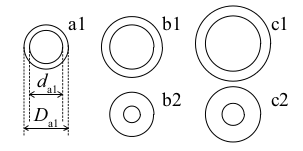
\includegraphics[scale=0.6]{Bilder/Theory/differentGeometries.png}
\caption{Different contact geometries \cite{bib:CIAMVLBS}} \label{fig:differentGeometries}
\end{figure}

It is expected that b2 and c2 will need a higher pressure than b1 and c1 to perform a successful interruption, due to the lower airflow. However it is expected that they will have an equal successrate no matter if the pin is inside the nozzle or outside the nozzle.
\newpage
\subsection{Interrupting currents} 
\subsubsection{Phenomenological description of a typical current interruption} \label{sec:InterruptCurrent}
A interrupting sequence in an AC power system have a typical pattern it follows. Under normal service the contacts are closed and current is flowing through the switchgear without electrical losses. Then a command signal to interrupt the current is sent to the breakers driving mechanism. The contacts is set to motion and a gap filled with an interrupting medium appears between them. An arc usually forms between the contacts and the current continues to flow trough the breaker. An electrical arc consists of plasma which is composed of electrons and other charge carriers like positive and negative ions. Due to energy dissipation in the arc the temperature of the plasma is generally quite high, but it is strongly dependent on the electrical current flow \cite{bib:HVEbreak}. In an AC power system the electrical current flow is mainly dependent on the sinus curve of the power cycle. Plasma with an high temperature tends to have a higher electric conductivity than plasma with an lower temperature. Electrical conductivity in an plasma channel is also strongly depend on the medium the plasma is burning in, the difference between air and SF${_6}$ will be discussed in section \ref{seq:airandsf}.

The arcing voltage, which is defined as the voltage drop over arc is dependent on the temperature and the cross-section of the arc \cite{bib:HVEbreak}, since these are depending on the current the arcing voltage can be regarded as constant. When the current approaches its zero crossing (CZ) the energy dissipation in the arc decreases and the plasma cools down. With different cooling mechanisms as mention in section \ref{sec:genDes} the breaker cools down the arc. If done sufficient the electric conductivity of interrupting medium becomes low, and it behaves as an isolator. This will quench the arc as the current amplitude reaches zero.

The moment after the arc have been quenched a voltage builds up over the contacts, this is called the recovery voltage \cite{bib:HVEbreak}. If a successful interruption is to occur, a re-ignition of the arc must be avoided as the recovery voltage increases. The probability of an re-ignition is set by the steepness and amplitude of the recovery voltage \cite{bib:HVEbreak}. There is two different kinds of re-ignition; it is the thermal and the dielectric re-ignition. The thermal re-ignition take place right after CZ and is mainly dependent on the recovery voltages steepness. As the recovery voltage rises and a thermal re-ignition is avoided a dielectric re-ignition may occur. This kind of re-ignition is largely dependent on the amplitude of the recovery voltage.

\subsubsection{Ionisation processes}
\subsubsection{Temperature profile for an electrical arc}

\subsubsection{The difference between air and SF$_6$ as interrupting medium} \label{seq:airandsf}
hva sskjer med ledeevnen naar den nearmer seg null, er hoey eller stigende? Dette maa diskuteres.
\newpage
\subsection{Environmental impacts of SF$_6$ from electrical power industries}
SF$_6$ is an effective infrared absorber and have a long lifetime in the atmosphere. This makes it a strong greenhouse gas. Because of the increase in commercial use since the 1970s the production of the gas have steadily increased. This have resulted in a rise of the SF$_6$ concentration in the atmosphere from barely measurable quantities in the 1980s \cite{bib:SF6PI} to sett inn nytt tall her!
\newpage

\begin{thebibliography}{10}


\bibitem{bib:HVEbreak} \textit{M. Runde}, \textit{Current Interruption in Power Grids}. Trondheim: Norwegian University of Science and Technology, 2013

\bibitem{bib:SF6PI} \textit{L.G. Christophorou, J. K. Olthoff, and R.J. Van Brunt}, "\textit{Sulfur Hexafluoride and the Electric Power Industry}", \textit{IEEE Electrical Insulation Magazine, vol. 13, No. 5, pp. 20-24}, Oct. 1997.

\bibitem{bib:comSub} \textit{amesimpex.com}, \url{http://www.amesimpex.com/images/unitised_sub_002.jpg}, \textit{26.9.2013}

\bibitem{bib:CIAMVLBS} \textit{E. Jonsson, N. S. Aanensen and M. Runde}, "\textit{Current Interruption in Air for a Medium Voltage Load Break Switch}", \textit{IEEE Trans. Power Delivery}, to be published.

\bibitem{bib:KlimaKur2020} "\textit{KLIMAKUR2020}", Oslo: Klima- og forurensningsdirektoratet, 2010

\bibitem{bib:CBAC} \textit{W. Rieder}, "\textit{Circuit breakers, Physical and engineering problems, III-Arc-medium considerations}", \textit{IEEE spectrum, pp. 80-84}, Sept. 1970.
\end{thebibliography}
\end{document}